\chapter{LHC y el detector ATLAS}

\section{LHC}

El Gran Colisionador de Hadrones (LHC, del ingles Large Hadron Collider) es el
acelerador de hadrones ubicado en el laboratorio CERN\footnote{CERN son las
  siglas en francés de \emph{Conseil Européen pour la Recherche Nucléaire}}, en
la frontera entre Francia y Suiza. Posee una longitud de 27 km y fue construido
en el mismo túnel en el que funcionaba el acelerador de electrones LEP entre
1989 y el 2000.

El LHC está diseñado para acelerar protones a 7 \tev, alcanzando energías de
centro de masa de 14 \tev, y una luminosidad de $10^{34}$ cm$^{-2}$s$^{-1}$. Uno
de los parámetros mas importantes para caracterizar el funcionamiento del
acelerador es la luminosidad instantánea (L), definida como el numero de
partículas por unidad de tiempo por unidad de área, que puede calcularse
mediante la relación:

\begin{equation}
  L = f_\text{rev} n_b \frac{N_1 N_2}{A}
\end{equation}
%
donde $f$ es la frecuencia de revolucion (sim 11 kHz), $n_b$ es el numero de
\emph{bunches} (paquetes de protones) por haz, $N_i$ es el numero de partículas
en cada bunch y A es la sección efectiva del haz, que puede expresarse en
termino de los parámetros del acelerador como:

\begin{equation}
  A = \frac{4\pi \epsilon_n \beta^{*}}{\gamma F}
\end{equation}
%
donde $\epsilon_n$ es la emitancia transversal normalizada (la dispersión
transversal media de las partículas del haz en el espacio de coordenadas e
impulsos), $\beta^{*}$ es la función de amplitud en el punto de interacción
(IP), relacionada al poder de focalización de los cuadrupolos), $\gamma$ es el
factor relativista de Lorentz y $F$ es un factor de reducción geométrico, debido
al ángulo de cruce de los haces en el IP.


Durante el año 2010, las colisiones se realizaron a 3.5 TeV por haz (7 TeV de
energía de centro de masa) y con una luminosidad que fue incrementándose hasta
alcanzar los $2 \times 10^{32}$ cm$^{-2}$ s$^{-1}$ en Octubre. %%\todo{complete
%%with 8 TeV run}

El diseño contempla trenes de 2808 paquetes de $\sim 10^{11}$ protones cada uno,
espaciados temporalmente en 25 ns.

Para acelerar los haces de protones y mantenerlos en sus orbitas circulares el
LHC cuenta con 1232 dipolos magnéticos superconductores que generan un campo
magnético de 8.4 T enfriados a 1.9 K. El sistema de focalización de los haces
consiste de 392 cuadrupolos magnéticos que generan campos magnéticos de 6.8 T.
Los haces circulan en direcciones opuestas en cavidades de ultra alto vacío
separadas a presión de 10$^{-10}$ torr.


\section{ATLAS}

ATLAS es un detector de partículas multipropósito del LHC diseñado y construido
para estudiar las colisiones protón-protón a una energía de centro de masa de
hasta 14 TeV. El nombre significa \textbf{A T}orodial \textbf{L}HC
aparatu\textbf{S}.

%% Los criterios básicos para el diseño del detector de ATLAS fueron:

%% \begin{itemize}
%% \item Un muy buen calorímetro electromagnético para la identificación y medidas de fotones y electrones, complementado con un calorímetro hadrónico para las medidas precisas de \emph{jets} y energía transversa perdida.
%% \item Medidas de alta precisión de momentos de muones, con la capacidad de garantizar mediciones precisas a la mas alta luminosidad usando sólo el espectrómetro de muones externo.
%% \item Alta eficiencia de la detección de trazas a alta luminosidad para medidas de momentos de leptones con alto \pt, identificación de electrones y fotones, identificación de $\tau$,  y capacidad de reconstrucción total de eventos con luminosidad baja.
%% \item Gran aceptancia en pseudorapidez ($\eta$) cubriendo casi todo el ángulo azimutal ($\phi$) en todo el detector.
%% \item Selección y medidas de partículas con bajo \pt, proveyendo alta eficiencia para la mayor parte de los procesos físicos de interés en el LHC.
%% \end{itemize}


El esquema general del detector se muestra en la figura \ref{fig:atlas}, donde
se señalan los componentes principales. ATLAS está diseñado en capas de
subdetectores que cumplen diferentes roles en la identificación de las
partículas producidas en las colisiones pp del LHC. Desde el punto de colision
hacia afuera ATLAS se compone de un ID subdividido a su vez en un detector de
píxeles (o capa B), un detector de bandas de silicio (SCT) y un detector de
radiación de transición (TRT).

\begin{figure}[H]
  \centering
  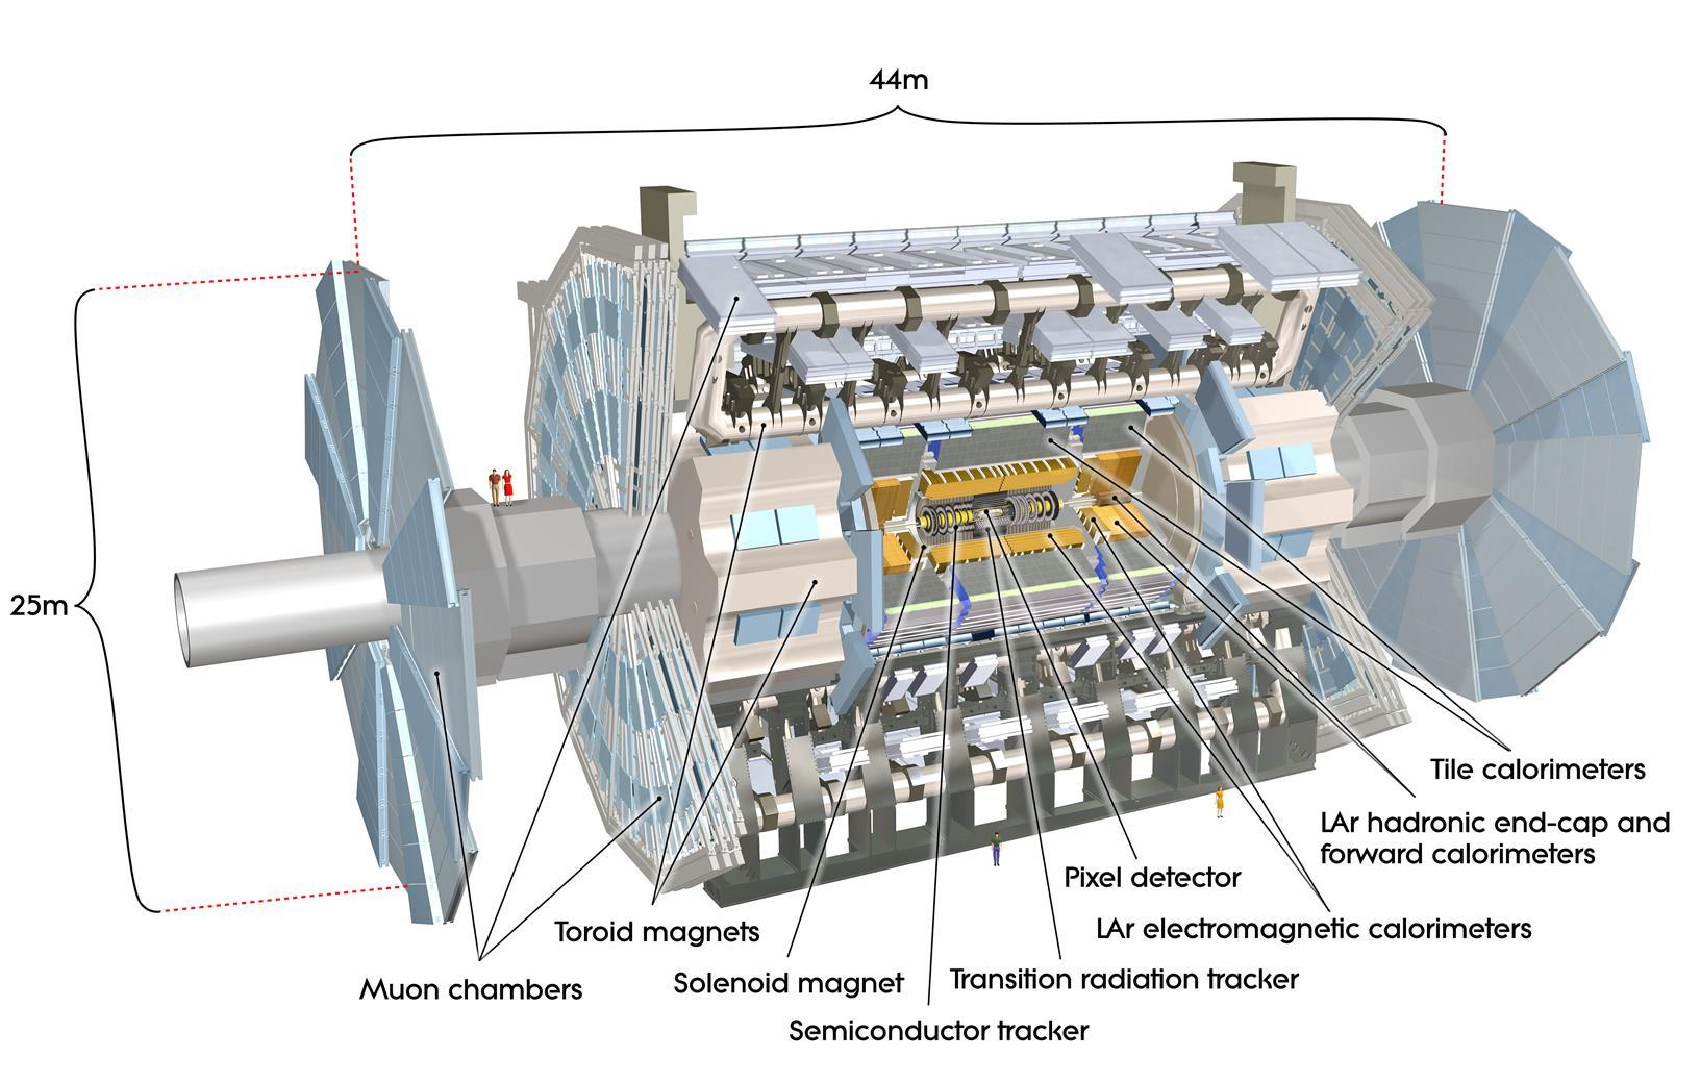
\includegraphics[width=0.85\textwidth]{figures/atlas}
  \caption{Esquema general del detector de ATLAS}\label{fig:atlas}
\end{figure}


Envolviendo este detector interno se encuentra un solenoide superconductor que
genera un campo magnético de $\sim$2 Tesla para que las partículas cargadas
curven su trayectoria. A continuación están ubicados los calorímetros: el
calorímetro electromagnético para medir la energía cinética de electrones y
fotones, y posteriormente el calorímetro hadrónico para medir la energía de los
\emph{jets} de hadrones.

En la capa más externa se encuentra el espectrómetro de muones que le da a ATLAS
el tamaño total de aproximadamente 45m de largo y más de 25m de alto.
Intercalado con éste se encuentra el sistema de toroides que genera el campo
magnético de $\sim$4 Tesla para curvar la trayectoria de los muones hacia el
final de su pasaje por el detector ATLAS.

El detector ATLAS se divide geométricamente en dos regiones, la región del
barril (la parte central, \emph{barrel}) y la región de las tapas (ambos
extremos, \emph{end-cap}). En cada una de estas regiones la ubicación de los
subdetectores es distinta. En la región del barril, los subdetectores están
ubicadas como cilindros concéntricos, mientras que en la región de las tapas
están ubicados como discos consecutivos.

\subsection{Sistema de coordenadas}

El sistema de coordenadas de ATLAS corresponde a un sistema cartesiano, cuyo
origen coincide con el punto de interacción nominal. El eje z es escogido,
naturalmente dada la concepción cilíndrica del detector, a lo largo del eje del
haz, en sentido antihorario. El eje $z$ positivo (negativo) define el lado A (C)
del detector, en vista de la simetría nominal del

mismo. El plano transversal $x-y$ es definido con valores positivos de $x$ e $y$
desde el origen en dirección hacia el centro del anillo del LHC y hacia la
superficie, respectivamente. Para describir la posición de los distintos
subdetectores y la trayectoria de las partículas dentro de ATLAS se utilizan
frecuentemente sistemas de coordenadas cilíndricas o polares. El radio R se
define como la distancia perpendicular al eje del haz. El ángulo azimutal $\phi
= 0$ corresponde al eje $x$ positivo y crece en sentido horario entorno al eje
$z$ positivo, mientras que el angulo $\theta$ se mide con respecto a este
ultimo. Una cantidad muy importante utilizada en física de altas energías es la
llamada rapidez:

\begin{equation}
  y = \frac{1}{2} \ln \left( \frac{E+p_z}{E-p_z} \right)
\end{equation}
%
donde E es la energia total de la particula y $p_z$ es la componente
longitudinal de su impulso. En el limite de altas energias esta cantidad se
aproxima (en forma exacta para objetos no masivos) por la llamada
\emph{pseudorapidez}, $\eta$, relacionada con el angulo polar $\theta$ como:

\begin{equation}
  \eta = - \ln \tan \left( \frac{\theta}{2} \right)
\end{equation}

La razon detras de esta transformacion de coordenadas es el hecho que la
multiplicidad de particulas producidas es aproximadamente constante como funcion
de $\eta$, y que la diferencia de pseudorapidez entre dos particulas es
invariante frente a transformaciones (boosts) de Lorentz a lo largo de la
direccion del haz. En el caso de colisiones hadronicas, la fraccion del impulso
del proton adquirida por cada uno de las partones interactuantes es desconocida;
parte de este impulso es transferido en la interaccion dura, mientras cierta
fraccion remanente escapa el detector a lo largo del haz. Asi, no es posible
reconstruir el movimiento longitudinal del centro de masa en la interaccion, y
aplicar leyes de conservacion sobre la cinematica de cada evento. Sin embargo,
dado que los protones inciden a lo largo de la direccion del haz, el impulso
total transverso es conservado durante la colision. Por esta razon, solo las
componentes transversales son utilizadas en la descripcion de la cinematica del
evento, e.g. $\et (= E \sin \theta)$ y $\pt (= p \sin \theta)$. En terminos de
la pseudorapidez, la energia transversa de una particula resulta:


\begin{equation}
  \et = \frac{E}{\cosh \eta}
\end{equation}
%
donde $E$ es su energia total.


\section{Los subdetectores de ATLAS}

A continuacion se describen brevemente cada uno de los subdetectores,
particularmente aquellos subsistemas utilizados para la identificacion de
electrones y fotones, pertinentes al analisis presentado en esta tesis.

\subsection{El detector interno}

El esquema del detector interno se muestra en la figura
\ref{fig:innerdetector}\cite{IDTDR}. Este sistema combina detectores de muy alta
resolución para distancias cortas al punto de interacción con detectores
continuos de trazas a distancias más lejanas. El detector interno está contenido
dentro del solenoide que provee un campo magnético nominal de 2T.

\begin{figure}[H]
  \centering \includegraphics[width=0.55\textwidth]{figures/figura}
  \caption{Esquema del detector interno}\label{fig:innerdetector}
\end{figure}

\subsubsection{Pixel}
Más cerca del punto de interacción se encuentra el detector de píxeles que se
compone de tres capas en el barril (a 4cm, a 10cm y a 13 cm del tubo del haz de
protones) y tres discos en cada tapa. Proveen mediciones de altísima precisión y
granularidad tan cerca del punto de interacción como es posible. El sistema
contiene en total 80 millones de elementos de 14x115 $\mu$m en (R$\phi$,z),
capaces de resolver la posición de las partículas mejor que 14$\mu$m.

\subsubsection{SCT}
Por fuera del detector de píxeles se encuentra el detector semiconductor de
trazas (SCT) que consta de ocho capas de detectores de micro bandas de silicio
que provee puntos de alta precisión en las coordenadas (R$\phi$,z). La
resolución espacial es de 16 $\mu$m en R$\phi$ y de 580 $\mu$m en z y tiene 6.2
millones de canales. Las trazas pueden distinguirse si están separadas más de
$\sim$200 $ \mu$m. El SCT cubre el rango de pseudorapidez de $|\eta|<$2.5.


\subsubsection{TRT}
La parte más externa del detector de trazas es el detector de radiación de
transición (TRT). Este detector está basado en el uso de detectores tubos que
pueden operar a alta frecuencia de eventos gracias a su pequeño diámetro (4mm) y
la aislación de sus hilos centrales en volúmenes de gas individuales.

El TRT además de detectar el pasaje de partículas cargadas, detecta la radiación
de transición que permite distinguir entre partículas cargadas pesadas y
livianas. La separación entre señales de trazas y de radiación por transición se
hace analizando tubo por tubo impactos de alto umbral e impactos de baja señal.
El largo de los tubos varía segun la zona del detector, llegando hasta los 144
cm en la zona del barril. El Barril contiene 50000 tubos y las tapas contienen
320000 tubos orientados radialmente. El número total de canales es de 420000 y
la resolución espacial es de 0.17mm.


\subsection{Calorímetros}

Una vista de los calorímetros de ATLAS puede verse en la figura \ref{fig:calo}.
Consiste en un calorímetro electromagnético cubriendo la región de pseudorapidez
$|\eta| < 3.2$, un calorímetro hadrónico en la sección \emph{barrel} cubriendo
la región $|\eta| < 3.2$, calorímetro hadrónicos en las \emph{end-cap} cubriendo
la región $1.5 < |\eta| < 3.2$, y calorímetros \emph{forward} cubriendo $3.1 <
|\eta| < 4.9$.

\begin{figure}[H]
  \centering \includegraphics[width=0.5\textwidth]{figures/figura}
  \caption{Esquema general del calorímetro del detector de
    ATLAS}\label{fig:calo}
\end{figure}


\subsubsection{Calorímetro electromagnético}
El calorímetro electromagnético \cite{caloemTDR} se divide en una parte central
(\emph{barrel}): $|\eta|<$1.475) y los extremos (\emph{end-caps}):
1.375$<|\eta|<$3.2. El barril está compuesto por dos mitades, separadas por una
distancia pequeña (6 mm) a $z = 0$. Las tapas del calorímetro están divididas en
dos ruedas coaxiales: una rueda externa cubriendo la región 1.375$<|\eta|<$2.5 y
una parte interna que cubre la región 2.5$<|\eta|<$3.2.

El calorímetro electromagnético es un detector de muestreo de Argón Líquido
(LAr) con electrodos de kaptón en forma de acordeón y planchas absorbentes de
plomo. El espesor total del calorimetro electromagnetico\ es $>$24 $X_0$ en el
barril y $>$26 $X_0$ en las tapas, ($X_0$ = longitud de radiación).

En la región dedicada a los estudios de física de precisión ($|\eta|<$2.5) el
calorímetro electromagnético está segmentado en tres secciones longitudinales.%
como se esquematiza en la figura \ref{fig:caloem}.

%\begin{figure}[H]
%  \centering
%  \includegraphics[width=0.85\textwidth]{./chapters/atlas/images/caloem}
%  \caption{Calorímetro Electromagnético del detector de ATLAS}\label{fig:caloem}
%\end{figure}


La sección de las bandas (\emph{strips}) que tiene un espesor constante de
$\sim$6 $X_0$ en función de $\eta$, está equipado con bandas finas de 4 mm de
largo en la dirección $\eta$. Esta sección actúa como un detector de pre-cascada
(\emph{pre-shower}) aumentando la capacidad de identificación de partículas,
(como por ejemplo la distinción entre $\gamma$ y $\pi_0$ o entre electrón y
$\pi^\pm$) y dando una precisa medición de la posición en $\eta$.

La sección del medio está segmentada transversalmente en torres cuadradas de
$\Delta \phi \times \Delta \eta=$0.025 $\times$ 0.025 (4 $\times$ 4 cm$^2$ en
$\eta=0$). El espesor total del detector hasta el final de la sección del medio
es $\sim$24$X_0$.

La sección mas externa tiene una granularidad de
$\Delta\phi\times\Delta\eta=$0.025 $\times$ 0.05 y su espesor varía entre 2 y 12
$X_0$.

\subsubsection{Calorímetro hadrónico}
El calorímetro hadrónico de ATLAS \cite{calohadTDR} cubre el rango $|\eta|<$4.9
usando diferentes materiales.

La parte del barril de este sistema consiste en un calorímetro de muestreo que
utiliza acero como absorbente y tejas centelladoras como material activo. Las
tejas están ubicadas radialmente y apiladas en profundidad.

%\begin{figure}[H]
%  \centering
%  \includegraphics[width=0.85\textwidth]{./chapters/atlas/images/calohad}
% \caption{Calorímetro Hadrónico del detector de ATLAS}\label{fig:calohad}
% \end{figure}

La estructura es periódica en z. Las tejas tienen un espesor de 3 mm y el
espesor de las placas de acero en un período es de 14 mm.

El calorímetro de tejas se extiende radialmente desde un radio interno de 2.28 m
hasta un radio externo de 4.25 m.

En la región de las tapas, el calorímetro hadrónico consiste en dos ruedas de
2.3 m de radio, perpendiculares al tubo del haz, hechas con placas de cobre y
tungsteno como material absorbente y argón líquido como material activo. Estos
detectores extienden la aceptancia del calorímetro de ATLAS hasta prácticamente
cubrir el ángulo sólido del punto de colisión.


\subsection{Espectrómetro de muones}
Los muones de alto {\pt} generados en el punto de interacción tienen un altísimo
poder de penetración y son poco interactuantes. Por ello el espectrómetro de
muones \cite{muonTDR} se encuentra situado en la parte más exterior del detector
ATLAS, alrededor del sistema de imanes de toroides, y está diseñado para obtener
mediciones de alta precisión de posición e impulso de muones de alto \pt.

\begin{figure}[H]
  \centering \includegraphics[width=0.7\textwidth]{figures/figura}
  \caption{Espectrómetro de muones del detector de ATLAS}\label{fig:especmuones}
\end{figure}

La figura \ref{fig:especmuones} muestra un esquema del espectrómetro de muones
de ATLAS. Es el subdetector más grande y el que le da a ATLAS su tamaño.

La región del barril está compuesta por tres capas concéntricas de cámaras de
trigger y de cámaras de precisión posicionadas a 5m, 7.5m y 10m del tubo del
LHC, cubriendo la región $|\eta|<1$. Las regiones de las tapas están compuestas
por cuatro capas de cámaras de trigger y cámaras de precisión a $|z|$= 7.4m,
10.8m, 14m y 21.5m cubriendo el rango de 1.0$<|\eta|<$2.7. Hay una pequeña
brecha en $|z|=0$ que permite el acceso de los servicios al ID.

%---------
% Trigger
%---------
\section{El sistema de Trigger}

Bajo las condiciones nominales de dise\~no del LHC, la tasa de interaccion
proton-proton en el LHC sera de $\mathcal{O}(1)$ GHz, considerando una
frecuencia de bunch crossing de 40 MHz y $\sim$ 23 interacciones por cruce. Dado
que la mayoria de los eventos son de baja energia y no son de interes para los
analisis mas relevantes en ATLAS, y tambien debido a las limitaciones de
almacenamiento y del poder de computo, el flujo de datos incidente debe ser
reducido al maximo permitido para su almacenamiento permanente ($\sim 200$ Hz).
El tamano tipico por evento es de $\sim 1.4$ MB, lo que resulta en un ancho de
banda requerido de $\sim 300$ MB/$s$. Esta reduccion se logra mediante una
rapida y eficiente preseleccion de eventso, conocida como \emph{trigger}. El
sistema de trigger de ATLAS [ref] esta organizado en tres niveles jerarquicos:
\emph{Nivel 1} (L1), \emph{Nivel 2} (L2) y \emph{Filtro de eventos} (EF), dondoe
los dos ultimos conforman el \emph{High Level Trigger} (HLT). Cada nivel permite
analizar los eventos con mayor detalle, aumentando la precision de los criterios
de seleccion y la complejidad de los algortimos utilizados. El sistema de
adquisicion de datos (DAQ) transfiere y almacena los datos seleccionados por el
trigger. La {\fig} {\XXX} muestra un esquema del sistema de Trigger-DAQ de
ATLAS.

El primer nivel del trigger se encarga de la seleccion inicial, reduciendo la
frecuencia de eventos que pasaran al siguiente nivel a $\sim 75$ kHz. Debido al
tamano limitado de las memorias temporales (buffers) donde se guardan los datos
de cada subdetector y al considerable tiempo de vuelo de las particulas hasta el
espctrometro de muones, la decision debe tomarse en una escala de tiempo muy
limitada ($2.5 \mu s$). El nivel 1 esta basado en hardware y selecciona objetso
de alto {\pt} construidos a partir de la informacion de varios subdetectores.
Los muones son identificados en las camaras de trigger descriptas en la sec XXX,
mientras que la informacion de los calorimetros, con una resolucion reducida, se
utiliza para identificar candidatos a electrones, fotones, jets y taus decayendo
hadronicamente. La posicion de cada objeto encontrado define una \emph{region de
  interes} (RoI) en un evento potencialmente interesante, que se extiende como
un cono desde el punto de interaccion a lo largo del detector.

En el calorímetro, el L1 se basa en las se\~nales analógicas obtenidas en cada
trigger tower (i.e. suma de celdas en una ventana $\Delta \eta \times \Delta
\phi = 0.1 \times 0.1$), definida separadamente para el ECAL y el HCAL (Fig.
3.7). El trigger de muones en el L1 utiliza las medidas de las trayectorias en
las diferentes estaciones de las cámaras de trigger: las RPCs en la región del
barrel y las TGCs en los endcaps. La aceptancia geométrica del L1 trigger esta a
ligada al dise\~no del detector, donde las medidas de precisión en los
calorímetros y la cobertura del detector interno están limitadas a la región
$\abseta < 2.5$. El trigger de fotones, electrones, muones y taus debe asegurar
la cobertura en esta región. En el caso del trigger de jets, las trigger towers
se extienden hasta $\abseta < 3.2$, mientras que para el calculo de la energía
transversa total (perdida) se utiliza todo el sistema calorimétrico (i.e.
$\abseta < 4.9$). Los resultados de los subsistemas del trigger son procesados
en el Central Trigger Processor (CTP), en donde se aplica una serie de
selecciones (\emph{menu}) definidas como una combinación de criterios
individuales, que pueden ser ajustados según la luminosidad y los requerimientos
físicos particulares de cada toma de datos. Un total de 256 configuraciones
(\emph{items}) estan disponibles en el L1, donde se programa el tipo de RoI (EM,
TAU, JET, etc.) y los umbrales de energía total y de aislamiento requeridos en
cada caso. Por ejemplo, el item L1EM14 acepta eventos donde al menos un (dos)
cluster(s) en el calorímetro electromagnético posee(n) $\et \geq 14 \GeV$.

El segundo nivel del trigger (L2) se centra unicamente en las RoIs donde el L1
encontro actividad, combinando informacion de todos los subdetectores dentro de
cada una ($\sim 2$ % de la cobertura total del detector). El L2 consiste de una
serie de algoritmos de reconstruccion y seleccion especializados, dise\~nados
para reducir la frecuencia de eventos hasta aproximadamente 1 kHz. Estos
algoritmos estan implementados en clusters de procesamiento dedicados (PC farms)
que analizan cada evento dentro de un tiempo de latencia medio de $\sim
\unit[40]{ms}$. El menor flujo de informacion en este nivel del trigger permite
calcular las variables calorimetricas con mayor precision y hacer uso de la
informacion de las trazas reconstruidas, haciendo posible la distincion entre
fotones y electrones, y el rechazo de fondo proveniente en su mayoria de jets.
13 En general, si bien la seleccion se basa en las mismas variables que la
identificacion offline descripta en la seccion 5.2 (sobre las caracteristicas de
las lluvias electromagneticas), los valores de corte en cada variable son
relajados (o a lo sumo igualados) respecto a la seleccion offline, para evitar
el rechazo prematuro de candidatos que satisfacen los criterios identificacion
durante el analisis final. La ultima etapa de la seleccion del trigger se lleva
a cabo en el Event Filter (EF), que reduce la frecuencia de eventos a $\sim
\unit[200]{Hz}$ ($\sim \unit[300]{MB/s}$). En este nivel se tiene acceso a toda
la informacion del evento en los distintos subdetectores de ATLAS, con la maxima
granularidad e incluyendo detalles sobre la calibracion de energia de los
calormetros, la alineacion de los subdetectores y el mapa de campo magnetico. El
tiempo de latencia relativamente largo disponible para tomar la decision final
sobre el evento ($\avg{t} \sim \unit[4]{s}$) permite la reconstruccion completa
del mismo, y el refinamiento de las variables y criterios de seleccion al nivel
de aquellos implementados en el analisis offline. Los eventos aceptados por el
EF son finalmente grabados a disco y distribuidos, accesibles offline para todos
los analisis subsecuentes.

Cabe mencionar que el sistema de TDAQ permite, en principio, una tasa de
procesamiento/almacenamiento por encima de estos parametros de dise\~no, por
periodos cortos de tiempo. Por ejemplo, durante el periodo de mas baja
luminosidad instantanea en el 2010 ($L\sim 10^{32} \text{cm}^{-2} s^{-1}$) se
alcanzaron frecuencias de lectura a la salida del EF de $\sim 600$ Hz, para
beneficiar los primeros analisis fisicos de ATLAS. Asimismo, el tiempo medio de
procesamiento por evento del EF fue de $\sim \unit[400]{ms}$, muy por debajo del
esperado. Al igual que en el Level 1, en cada nivel del HLT se configuran
ciertos criterios (\emph{signatures}) segun el tipo y multiplicidad de la
particula que se busca en el evento, y el conjunto de cortes de identificacion
aplicados. La nomenclatura adoptada como convencion en el trigger de ATLAS tiene
la forma general L ipX Y, donde L es el nivel del trigger (L2,EF), i la
multiplicidad, p la particula de interes (e.g. g=foton, e=electron), X el {\pt}
minimo requerido e Y el tipo de identificacion aplicada (loose, tight, etc.
segun se describe en la Sec. 5.2). 14 Las signatures del L2/EF y su item
asociado en el L1 (i.e. el que pasa las RoI al L2) definen en conjunto una de
las \emph{cadenas} del trigger, que toman el nombre de la signature del HLT
(i.e. ipX Y segun la convencion anterior) y conforman el \emph{menu} final del
trigger.


Para cada item (signature) del trigger a Level 1 (L2/EF) se puede asignar ademas
un factor de escala o prescale (PS), que define la frecuencia con la que un dado
item/signature es evaluado por el trigger (i.e. solo en uno de cada PS eventos).
Se habla de una cadenade trigger \emph{unprescaled} si su factor de escala es
PS=1 en cada nivel (i.e. si es evaluada evento a evento). La asignacion de estos
factores se hace incluso dinamicamente durante una toma de datos, para tener en
cuenta el descenso de la luminosidad instantanea con el tiempo y mantener la
tasa de procesamiento aproximadamente constante.


\section{Modelo computacional y distribución de datos}

El modelo computacional de ATLAS esta diseñado para permitir a todos los
miembros de la colaboración un acceso ágil, directo y distribuido a la gran
cantidad de datos colectados por el detector ($\sim \text{PB}/\text{a\~no}$),
así como a las diversas simulaciones MC. El modelo se basa en la tecnología
GRID, compartiendo el poder de procesamiento y la capacidad de almacenamiento
disponibles en distintos centros de computo asociados alrededor del mundo. El
software de ATLAS se desarrolla dentro un entorno C++ común llamado
\texttt{ATHENA} [104–106], basado en el projecto GAUDI [107]. Todo el
procesamiento de los datos en ATLAS se realiza dentro de este entorno,
incluyendo la implementación y configuración del HLT, la simulación de la
respuesta del detector, la generación de las muestras MC de los distintos
procesos físicos, y la reconstrucción y análisis de los datos. Los eventos
aceptados por el trigger deben ser procesados para reducir su tamaño y ser
utilizados para los análisis offline. A la salida del EF, los eventos son
almacenados como Raw Data Objects (RDOs). Luego de aplicar los algoritmos de
reconstrucción y calibración, las colecciones de los distintos objetos físicos
obtenidas (fotones, electrones, etc.) son almacenadas en formato ESD (Event
Summary Data) y AOD (Analysis Data Object), una versión reducida del primero
($\sim 100$ kB/evento). A partir de las ESDs/AODs, se ha definido un formato de
datos significativamente mas pequeño (10-15 kB/evento) conocido como D3PD
(Derived Physics Data), sobre el que se realiza el análisis final. Las D3PDs son
archivos (\emph{ntuples}), accesibles vía el entorno de análisis de datos ROOT
[108], que contienen un conjunto de variables para diferentes objetos físicos,
según las necesidades de cada grupo de análisis dentro de ATLAS. Para el
análisis de esta tesis, se utilizaron las D3PDs definidas y producidas en forma
centralizada por el SM Direct Photon group. La misma cadena de reconstrucción y
distribución se aplica a las simulaciones Monte Carlo, a fin de conservar un
modelo de análisis único y garantizar la consistencia en la comparación de estas
con los datos experimentales.


\section{Datos de colisiones $pp$ a $\sqrt{s} = 8$ \tev}

El presente análisis se basa en el conjunto de eventos colectados de las
colisiones $pp$ a una energía de centro de masa $\sqrt{s} = 8\tev$ con el
detector ATLAS en 2012.

Estos corresponden a una luminosidad integrada $\int L dt = 20.3 \pm 0.7 \ifb$
\cite{lumi2012}
%% after the application of beam, detector and data quality requirements \footnote{GRL \texttt{data12\_8TeV.periodAllYear\_DetStatus-v61\-pro14\-02\_DQDefects\-00\-01\-00\_PHYS\_StandardGRL\_All\_Good.xml}}.
%% The collected integrated luminosities split up by run period is shown in {\tab} \ref{tab:data_periods}.
%% The data sample is collected by a single photon trigger (\trigchain) with a transverse momentum threshold of 120 \gev, which selects events with at least one photon passing the loose identification criteria. This trigger has been kept unprescaled through the whole data taking, and is fully efficient selecting photons with $p_{T}>125 \gev$ accepted by the signal selection cuts described in {\sec} \ref{sec:event_selection}. The trigger efficiency extraction and the uncertainty evaluation is treated in {\sec} \ref{sec:trigger_eff}.

\begin{table}[ht]
  \centering
  \caption{Luminosidad integrada de cada periodo de toma de datos de colisiones
    $pp$ a una energía de centro de masa de $8 \tev$ utilizada en este
    análisis.}
  \begin{tabular}{c|c|r}
    \hline \hline Periodo & \emph{Runs} & Luminosidad $[\ipb]$ \\
    \hline \hline
    A & 200804--201556 & 795.91 \\
    B & 202660--205113 & 5113.61 \\
    C & 206248--207397 & 1409.06 \\
    D & 207447--209025 & 3297.54 \\
    E & 209074--210308 & 2534.11 \\
    G & 211522--212272 & 1279.54 \\
    H & 212619--213359 & 1449.04 \\
    I & 213431--213819 & 1018.45 \\
    J & 213900--215091 & 2605.48 \\
    L & 215414--215643 & 841.634 \\
    \hline \hline
    Total & 200804--215643 & 20344.37 \\
    \hline \hline
  \end{tabular}
  \label{tab:data_periods}
\end{table}



%% 2 ATLAS Offline Software Overview
%% The ATLAS software framework, Athena [3], uses Python
%% as an object-oriented scripting and interpreter language
%% to configure and load C++ algorithms and objects.
%% Rather than develop an entirely new high-energy physics
%% data processing infrastructure, ATLAS adopted the Gaudi
%% framework [6, 7], originally developed for LHCb and written
%% in C++. Gaudi was created as a flexible framework to
%% support a variety of applications through base classes and
%% basic functionality. As much as possible, the infrastructure
%% relies on the CLHEP common libraries [8], which include
%% utility classes particularly designed for use in high-energy
%% physics software (e.g. vectors and rotations).
%% Athena releases are divided into major projects by
%% functionality [9], and all of the ATLAS simulation software
%% (including event generation and digitization) resides
%% in a single project. The dependencies of the “simulation”
%% project are the “core” project, which includes the Athena
%% framework, the “conditions” and “detector description”
%% projects, which include all code necessary for the description
%% of the ATLAS detector, and the “event” project,
%% which includes descriptions of persistent objects. The number
%% of lines of code by software language for the simulation
%% project are summarized in Table 1, as calculated using
%% cloc [10] in Athena release 14.4. Lines of code in the upstream
%% Athena projects, excluding external dependenccies
%% like Gaudi and CLHEP, are summarized in Table 2.
